\documentclass[10pt,twocolumn,twoside,final]{IEEEtran}

% cite package, to clean up citations in the main text. Do not remove.
\usepackage{cite}
\usepackage{lastpage,fancyhdr,graphicx}
\usepackage{amssymb,amsmath}

\bibliographystyle{plain}

% Remove brackets from numbering in List of References
\makeatletter
\renewcommand{\@biblabel}[1]{\quad#1.}
\makeatother

% *** SUBFIGURE PACKAGES ***
\ifCLASSOPTIONcompsoc
  \usepackage[caption=false,font=footnotesize,labelfont=sf,textfont=sf]{subfig}
\else
  \usepackage[caption=false,font=footnotesize]{subfig}
\fi

\begin{document}

\title{Effective Dynamic Models of Metabolic Networks}


% author names and affiliations
% use a multiple column layout for up to three different
% affiliations
\author{\IEEEauthorblockN{Michael Vilkhovoy\IEEEauthorrefmark{1},
Mason Minot\IEEEauthorrefmark{2},
Jeffrey D. Varner\IEEEauthorrefmark{1}}\\
\IEEEauthorblockA{\IEEEauthorrefmark{1}School of Chemical Engineering, Purdue University, West Lafayette, IN 47907 USA}
\IEEEauthorblockA{\IEEEauthorrefmark{2}School of Chemical and Biomolecular Engineering, Cornell University, Ithaca, NY 14850 USA}
\thanks{Manuscript received December 1, 2012; revised September 17, 2014.
Corresponding author: J. Varner (email:jdvarner@purdue.edu).}}

\maketitle

\begin{abstract}
Mathematical models of biochemical networks are useful tools to understand and ultimately predict how cells utilize nutrients to produce valuable products.
Modified version of the last paragraph of the introduction. Mike made this change.

\end{abstract}


\begin{IEEEkeywords}
Dynamic metabolic models, flux balance analysis, cybernetic models
\end{IEEEkeywords}

\section{Introduction}
Three paragraphs, all must fit (along with abstract) on the first page.
First, introduce the need to model and unstructured, structured, cybernetic, and recent palsson dynamic models of biochemical networks.
Second paragraph introduce constraints based modeling, and its modifications along with EMs. Stress the issues with calculating EMs for large networks. Ref the parallel work.
Third paragraph summarize what you have done. This paragraph must start with ``In this study, we developed a ... ''. It describes what you did, what the results were and what big picture conclusions you have drawn from the study. Last like should start with ``Taken together, ... ''. Always past tense. We did this, we saw that. SIMPLE LANGUAGE, SHORT DECLARATIVE SENTENCES.


\begin{figure}[!t]\centering
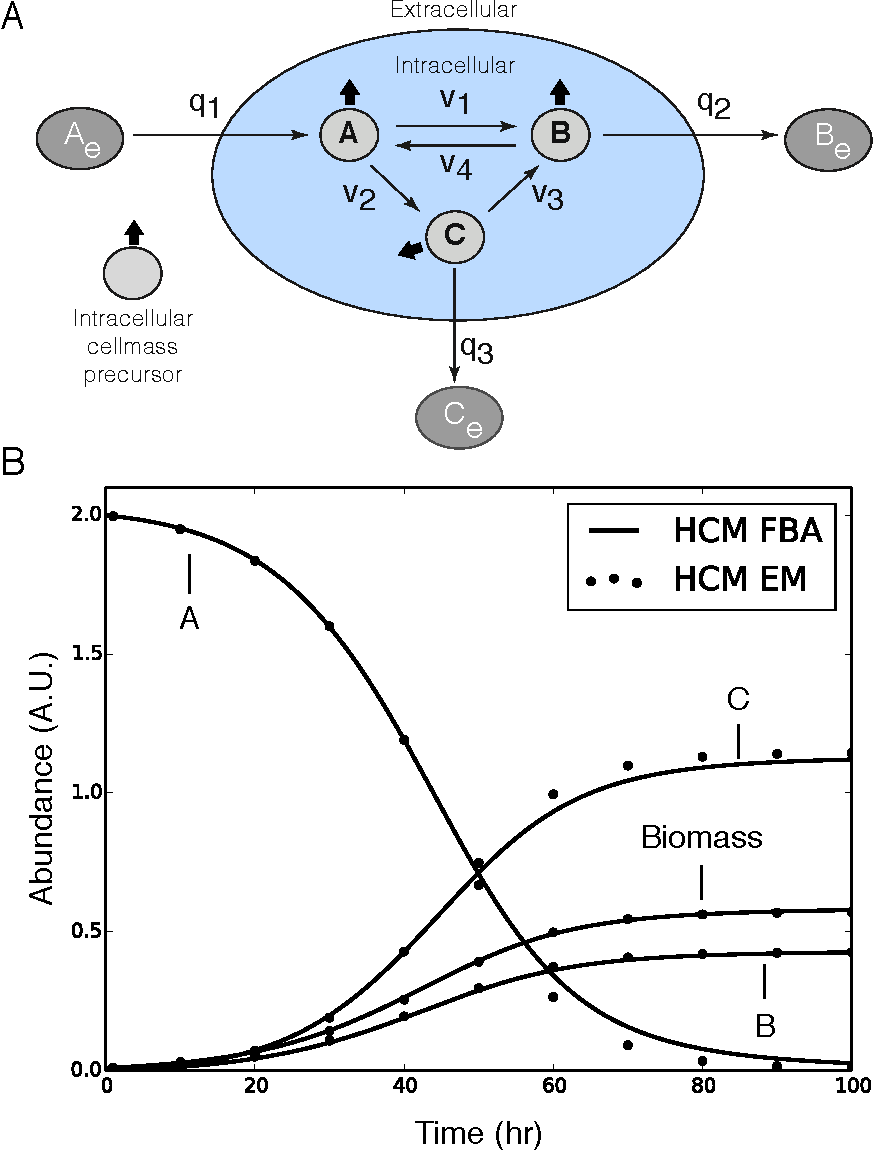
\includegraphics[width=0.40\textwidth]{./figs/Fig-1-GeneralModel-Results.pdf}
\caption{A: Proof of concept metabolic network with six metabolites and seven reactions.
Intracellular cellmass precursors $A,B$ and $C$ are balanced (no accumulation) while the extracellular metabolites ($A_{e},B_{e}$ and $C_{e}$) are not balanced (can accumulate). The blue-oval denotes the cell boundary, where $q_{j}$ denotes the jth flux across the boundaries ([mmol/gdw-hr]) and $v_{k}$ denotes the kth intracellular flux. B: Simulation of the extracellular metabolites using the FBA hybrid cybernetic approach (solid line) versus elementary modes (points) for the proof of concept metabolic network. FBA modes have comparable model performance compared to elementary modes.
}\label{fig:model-fitting}
\end{figure}

\section{Results}
In the general case model, we demonstrated that the performance of the hybrid cybernetic model with FBA modes was equivalent to that of the elementary modes. In the proof of concept metabolic network consisting of 6 metabolites and 7 reactions (Fig. \ref{fig:model-fitting} A), METATOOL generated 6 elementary modes. FBA generated 3 possible modes (pathways) for the same metabolic network. Temporal profiles of the extracellular metabolites and artificial biomass concentration are presented for both the HCM FBA and HCM EM models (Fig. \ref {fig:model-fitting} B).  HCM FBA has 9 kinetic parameters whereas HCM EM has 15 kinetic parameters. The kinetic parameters of HCM FBA were varied to fit the concentration profiles of the HCM EM model. 

General case = we showed that EMs and FBA models were equivalent for the small hypothetical model

Small E. coli case = we should that EMs and a fewer number of FBA models gave similar model performance

Large E. coli case = too many EMs, small number of FBA modes allowed us to simulate this network opening up the possibility of genome scale cybernetic models.

Sensitivity results = simple systematic method to eliminate FBA modes to give the smallest number needed, without complex weighting schemes.

In all cases, the first line of the paragraph states the result described in the paragraph. All results are in past tense.



\section{Discussion}
Three paragraphs.
First paragraph, modified version of the last paragraph of the introduction, more details.

Second paragraph, contrast what we have done in the context of the field, in particular compare the hybrid cybernetic models, constraints based models and dynamic models of
Palsson. Why is this study innovative?

Last paragraph, what is wrong with this study and where do we go from here? For example,
could we extend the work done here to animal cells producing biologics, could we extend this to genome scale.

\section{Materials and Methods}

\noindent\subsubsection*{Description of the method}
Describe the method mathematics, use index form if possible, I the vector nomenclature to be hard to follow. Define all terms and symbols.

\subsubsection*{Estimation of model parameters Modify this section}
Model parameters were estimated by minimizing the difference between simulations and experimental thrombin measurements (squared residual):
\begin{equation}\label{eqn:objective-function}
	\min_{\mathbf{k}} \sum_{\tau=1}^{\mathcal{T}}\sum_{j=1}^{\mathcal{S}}\left(\frac{\hat{x}_{j}\left(\tau\right) - x_{j}\left(\tau,\mathbf{k}\right)}{\omega_{j}\left(\tau\right)}\right)^{2}
\end{equation}where $\hat{x}_{j}\left(\tau\right)$ denotes the measured value of species $j$ at time $\tau$, $x_{j}\left(\tau,\mathbf{k}\right)$ denotes the simulated
value for species $j$ at time $\tau$, and $\omega_{j}\left(\tau\right)$ denotes the experimental measurement variance for species $j$ at time $\tau$.
The outer summation is with respect to time, while the inner summation is with respect to state. We minimized the model residual using Particle swarm optimization (PSO) \cite{PSO}. PSO uses a \textit{swarming} metaheuristic to explore parameter spaces.
For each iteration, particles in the swarm compute their local error by evaluating the model equations using their specific parameter vector realization.
From each of these local points, a globally best error is identified. Both the local and global error
are then used to update the parameter estimates of each particle using the rules:
\begin{eqnarray}
	\mathbf{\Delta}_{i} &=&\theta_{1}\mathbf{\Delta}_{i} + \theta_{2}\mathbf{r}_{1}\left(\mathcal{L}_{i} - \mathbf{k}_{i}\right) + \theta_{3}\mathbf{r}_{2}\left(\mathcal{G} - \mathbf{k}_{i}\right) \\
	\mathbf{k}_{i} &=& \mathbf{k}_{i} + \mathbf{\Delta}_{i}
\end{eqnarray}where $\left(\theta_{1},\theta_{2},\theta_{3}\right)$ are adjustable parameters, $\mathcal{L}_{i}$ denotes the local best solution found by particle $i$, and
$\mathcal{G}$ denotes the best solution found over the entire population of particles. The quantities $r_{1}$ and $r_{2}$ denote uniform random vectors with the same dimension as the number of unknown model
parameters ($\mathcal{K}\times{1}$). In thus study, we used $\left(\theta_{1},\theta_{2},\theta_{3}\right) = \left(1.0, 0.05564, 0.02886\right)$. The quality of parameter
estimates was measured using goodness of fit (model residual). The particle swarm optimization routine was implemented in the Python programming language.

% References -
\bibliography{Paper_v1}

\end{document}
